\documentclass[12pt]{article}
\usepackage{amsmath}
\usepackage{amssymb}
\usepackage{graphicx}
\begin{document}
\title{Computer Science 143, Homework 4}
\date{June 1st, 2018}
\author{Michael Wu\\UID: 404751542}
\maketitle

\section*{Part 1}

\subsection*{Problem 1}

Yes, this is a lossless decomposition. Since \(A\rightarrow BC\) and \(B\rightarrow D\), we have that \(A\rightarrow BCD\). Then
since \(CD\rightarrow E\), we have that \(A\rightarrow BCDE\). So \(A\rightarrow ADE\), and \(A\) is a superkey for \(R_2\). Since
\(R_1 \cap R_2 = \{A\}\), we have \(R_1 \cap R_2 \rightarrow R_2\).

\subsection*{Problem 2}

\[\{A\rightarrow B, C\rightarrow B, C\rightarrow A\}\]

\subsection*{Problem 3}

\paragraph{a)}

Yes. We have that \(E\rightarrow A\) and \(A\rightarrow BC\), so \(E\rightarrow ABC\). Then we have \(B\rightarrow D\), so \(E\rightarrow ABCD\).
Along with the trivial functional dependency \(E\rightarrow E\), we get \(E\rightarrow ABCDE\) or \(E\rightarrow R\). Thus \(E\) is a key for \(R\).

\paragraph{b)}

Yes. We have the trivial functional dependency \(BC\rightarrow BC\) and \(B\rightarrow D\), so \(BC\rightarrow BCD\). Then we have \(CD\rightarrow E\),
so \(BC\rightarrow BCDE\). Finally we have \(E\rightarrow A\), so \(BC\rightarrow ABCDE\), or \(BC\rightarrow R\). Thus \(BC\) is a key for \(R\).

\subsection*{Problem 4}

This is not in BCNF. Consider the functional dependency \(B\rightarrow D\). The dependency \(B\rightarrow F\) cannot be derived from the closure of the
set of funtional dependencies, so \(B\) is not a key for \(R\). Thus there exists some nontrivial functional dependency in \(R\) where the left hand side
is not a key for \(R\). If it was in BCNF, this could not happen. To normalize it into BCNF, decompose it into the relations \(R_1(A,F)\), \(R_2(A,B,C)\),
\(R_3(C,E)\), and \(R_4(B,D)\).

\subsection*{Problem 5}

\begin{multline*}
        \{(a,b_1,c_1,d_2),(a,b_1,c_1,d_3),(a,b_2,c_2,d_1),\\
        (a,b_2,c_2,d_3),(a,b_3,c_3,d_1),(a,b_3,c_3,d_2)\}
\end{multline*}

\subsection*{Problem 6}

No it is not in 4NF. We have a nontrivial multivalue dependency \(A\twoheadrightarrow B\) where \(A\) is not a key, which violates the
conditions of 4NF. To normalize it into 4NF, decompose it into the relations \(R_1(A,D,F)\), \(R_2(A,B)\), \(R_3(A,C)\), and \(R_4(A,E)\).

\pagebreak

\section*{Part 2}

\subsection*{Problem 1}

\begin{figure}[!ht]
    \begin{center}
        \hspace*{-5cm}
        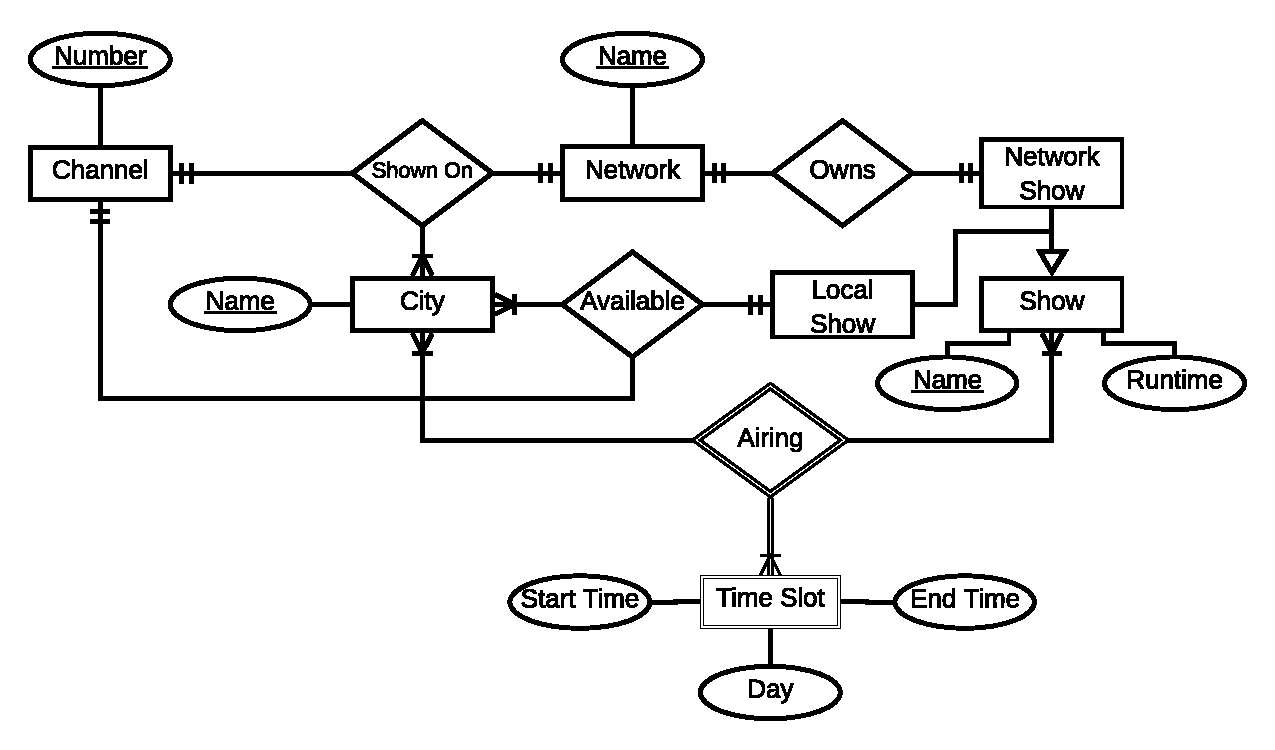
\includegraphics[width=1.25\textwidth]{problem2-1.pdf}
        \hspace*{-5cm}
    \end{center}
\end{figure}
Some assumptions I made were that a given show could only be shown on one channel in a given city, and a network could only be associated with one
channel in a given city. Multiple cities can have a given network on a given channel, and multiple cities can have a given show on a given channel.
I used subclasses to represent the distiction between a network show and a local show. With these relationships, one can determine the channel
that a show will be shown on. Separate from this, there is a weak entity set called ``Time Slot'' which allows us to determine when shows are shown
in a given city. A show may be shown multiple times for a given city, a city may have multiple shows showing in a given time slot, and a show may
have multiple cities that it's showing in for a given timeslot. Thus all the arrows in this relationship set are many to many.

\subsection*{Problem 2}

This can be converted into the three relations shown below.
\begin{center}
        assembly(\underline{number}, name, cost)\\
        parts(\underline{number}, name)\\
        composed\_of(\underline{assembly\_number}, parts\_number, quantity)
\end{center}
In these tables, assembly\_number is a foreign key that references the key of assembly, and parts\_number is a foreign key that references the key of parts.

\section*{Part 3}

\subsection*{Problem 1}

\begin{figure}[!ht]
    \begin{center}
        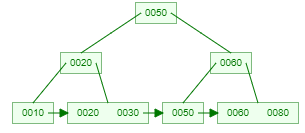
\includegraphics{problem3-1.png}
    \end{center}
\end{figure}

\subsection*{Problem 2}

\begin{figure}[!ht]
    \begin{center}
        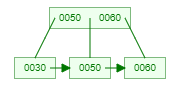
\includegraphics{problem3-2.png}
    \end{center}
\end{figure}

\end{document}